\section{Què és?}

El software lliure (de l'anglès \emph{"free software"}) és tot aquell software publicat
sota llicències que respecten el concepte de \emph{llibertat}. Degut a que la definició
(en relació al software) de llibertat és molt àmplia, i es podria dedicar inacabable espai
a definir-la, utilitzarem la definició més acceptada, la que ha popularitzat la \ac{fsf}; \emph{un programa és lliure si al adquirir-lo, l'usuari pot fer-lo servir,
copiar-lo, estudiar-lo, modificar-lo, i redistribuir-lo lliurement de diferents formes}. \cite{wikifree}

Que el software sigui lliure, no implica que el seu cost sigui zero (encara que molt
software lliure, també sigui gratuït) \cite{sellingfree}. Per tant, jo puc crear software lliure i distribuir els arxius
binaris a \EUR{500,000}, mentre mantingui un lliure accés al codi font. El desenvolupament de software
lliure es sol finançar a través de donacions voluntàries, i la major part de projectes dediquen
aquests diners recaptats al manteniment dels serveis que el software que distribueixen necessita
(cost dels servidors i manteniment web, etc).

\section{Qui el fa?}

La major part de software lliure no és realitzat per companyies multimilionàries; en canvi,
petits i mitjans grups de desenvolupadors són qui donen vida a la gran comunitat de software lliure.
Tot i això, la major part de projectes de software lliure relativament importants
són suportats i actualitzats per empreses que no es dediquen exclusivament a \emph{crear}
software lliure, però que n'utilitzen, i això les motiva a millorar-lo (per exemple, \emph{HP, IBM, Intel, Oracle, Samsung, AMD, Google, Cisco, Toyota, Panasonic, Adobe, Dell, Epson, LG, Nokia, Nissan, Nvidia, Sony, Siemens, Toshiba, Yahoo...}\cite{linuxmembers}).

Definir la importància del software lliure basat en el nombre d'empreses que hi col·laboren no és la forma més correcta de fer-ho; hi han milers de programadors que actualitzen programari lliure cada dia, molts d'ells de forma altruista, i això no incrementa el nombre d'empreses.

La comunitat de software lliure és extremadament viva, i omple tots els tipus de programari que un usuari pugui desitjar. Per exemple; el projecte \emph{Linux} accepta setmanalment un mitja de 750 col·laboracions en el seu codi font, i té més de 3,500 col·laboradors actius \cite{linuxgitrepo}. El reproductor de vídeo i audio \emph{VLC} (un projecte més petit, que Linux, evidentment), té una mitja de 200 col·laboracions setmanals \cite{vlcgitrepo}. Dia a dia, desenvolupadors individuals o grups reduïts utilitzen diferents plataformes a internet per a iniciar els seus projectes de software lliure, i permetre la col·laboració amb molts més programadors.

\section{Història}

Des dels anys 50 fins als 70, no hi havien grans corporacions que 
llicenciessin software, i es solia compartir de forma lliure entre
programadors, i distribuir de forma integrada en el \emph{hardware}
(es a dir, els ordinadors). Una vegada entrats en els 70, la indústria del
software va començar a mostrar la seva capacitat econòmica, i es va
començar a vendre programari per separat. \cite{ibmusdata}

En \emph{Richard Matthew Stallman}, va anunciar el projecte \emph{GNU} (\emph{GNU no és Unix!}, conjunt d'utilitats per a iniciar un sistema operatiu lliure), argumentant que s'havia cansat dels efectes del canvi en la cultura de la indústria informàtica i els seus usuaris. La FSF (\emph{Free Software Foundation}) va ser fundada l'Octubre de 1984, i va desenvolupar una de les definicions de \emph{software lliure} més acceptades, i el concepte de \emph{copyleft}, dissenyat per a assegurar la llibertat de software per a tothom. \cite{fossieee}.

A partir d'aquell moment, la comunitat de software lliure va començar a créixer.

\begin{figure}[ht!]
\centering

\includegraphics[width=100mm]{data/fsf.png}
\caption{El logotip de la \ac{fsf}.}
\label{fsfpic}
\end{figure}

\section{Us actual}

En l'actualitat, hi ha molt software lliure en circulació activa, i una gran comunitat de desenvolupadors darrere d'ell, però no és tant popular com el software propietari (que no vol dir que no sigui utilitzat tant).

No només els usuaris particulars tenen a l'abast (i utilitzen) software lliure: molts governs han fet (o estan fent) el traspàs al software d'aquest tipus (Kerala, a la Índia, Munich, a Alemanya, Veneçuela, Malàisia, Perú, Equador, i altres). \cite{fossadopters}

\section{Avantatges i inconvenients}

El software lliure té una quantitat important d'avantatges  \cite{fossadvantages}:

\begin{enumerate}
\item \emph{Econòmic} - molta part del FOSS (software de codi obert i lliure) és gratuït, o té un preu molt baix. Les petites empreses es poden beneficiar d'això, i expandir la seva infraestructura informàtica sense gastar milers d'euros en software propietari.
\item \emph{Llibertat d'ús i distribució} - es pot instal·lar software lliure sense limitacions per culpa de llicències d'un sol ús, com passa amb els sistemes operatius i 'suites' ofimàtiques.
\item \emph{Independència tecnològica} - l'accés al codi font permet desenvolupar nous productes amb una base sòlida de software, o ajustar-lo a les nostres necessitats. Quan s'utilitza software lliure, no s'ha de patir per les decisions de l'entitat creadora, ja que sempre es tindrà accés a versions més antigues, o en casos més avançats, al codi font.
\item \emph{Sistemes sense 'backdoors'} - tenir accés al codi impossibilita la implementació de \emph{espies} en el codi font d'un programa.
\item \emph{Correcció més ràpida i eficient d'errors} - la comunitat activa de desenvolupadors de software lliure realitzen actualitzacions constants, i errors o 'bugs' són arreglats molt més ràpid que en el software propietari.
\end{enumerate}

De totes formes, també té desavantatges \cite{gentegeek}:

\begin{enumerate}
\item \emph{Falta de garantia} - el software lliure no ofereix garanties; si es trenca, no és culpa de ningú excepte teva, si es que has fet alguna cosa malament.
\item \emph{Difícil d'adquirir} - hi ha una certa quantitat de software lliure que és més complicat de descarregar i instal·lar en comparació amb el seu germà propietari. Es deu, en molts casos, en que els autors es centren en el \emph{codi} del programa, i no tenen els recursos suficients per assegurar la disponibilitat de paquets compilats per a cada plataforma.
\item \emph{Acabat final} - molt software lliure ofereix un aspecte gràfic o final poc atractiu; no hi han equips dedicats íntegrament al desenvolupament de l'interfície gràfica, i es fa el que es pot, amb els recursos que es tenen.
\item \emph{Entreteniment} - els títols \emph{AAA} (jocs amb pressupost molt elevat) no són lliures. Falta molt de temps per a que l'usuari comú pugui observar l'impressionant codi font de títols com \emph{Battlefield} o \emph{Far Cry}, ja que el mercat és més lucratiu que ètic, i s'hi troben molts inconvenients en alliberar el codi font d'un \emph{engine} (motor gràfic).
\end{enumerate}

\begin{figure}[ht!]
\centering
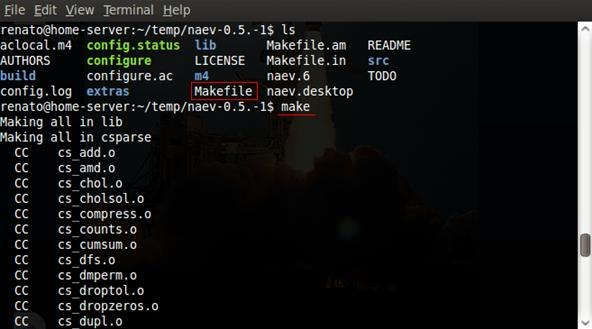
\includegraphics[width=100mm]{data/linuxcompile.jpg}
\caption{Procés de compilació de Linux (\href{http://renatonel.wonderhowto.com/inspiration/first-steps-compiling-program-linux-0127658/}{wonderhowto.com}).}
\label{websshare}
\end{figure}